\documentclass[journal]{IEEEtran}

  \usepackage{graphicx}
  \usepackage{fixltx2e}
  \usepackage{stfloats}
  \usepackage{listings}
  \usepackage{caption}

  \usepackage{tikz}
  \usetikzlibrary{shapes.multipart}  
  
  \usepackage{pgfplots}


\pgfplotsset{
    box plot/.style={
        /pgfplots/.cd,
        black,
        only marks,
        mark=-,
        mark size=0.2em,
        /pgfplots/error bars/.cd,
        y dir=plus,
        y explicit,
    },
    box plot box/.style={
        /pgfplots/error bars/draw error bar/.code 2 args={%
            \draw  ##1 -- ++(0.2em,0pt) |- ##2 -- ++(-0.2em,0pt) |- ##1 -- cycle;
        },
        /pgfplots/table/.cd,
        y index=2,
        y error expr={\thisrowno{3}-\thisrowno{2}},
        /pgfplots/box plot
    },
    box plot top whisker/.style={
        /pgfplots/error bars/draw error bar/.code 2 args={%
            \pgfkeysgetvalue{/pgfplots/error bars/error mark}%
            {\pgfplotserrorbarsmark}%
            \pgfkeysgetvalue{/pgfplots/error bars/error mark options}%
            {\pgfplotserrorbarsmarkopts}%
            \path ##1 -- ##2;
        },
        /pgfplots/table/.cd,
        y index=4,
        y error expr={\thisrowno{2}-\thisrowno{4}},
        /pgfplots/box plot,
    },
    box plot bottom whisker/.style={
        /pgfplots/error bars/draw error bar/.code 2 args={%
            \pgfkeysgetvalue{/pgfplots/error bars/error mark}%
            {\pgfplotserrorbarsmark}%
            \pgfkeysgetvalue{/pgfplots/error bars/error mark options}%
            {\pgfplotserrorbarsmarkopts}%
            \path ##1 -- ##2;
        },
        /pgfplots/table/.cd,
        y index=5,
        y error expr={\thisrowno{3}-\thisrowno{5}},
        /pgfplots/box plot
    },
    box plot median/.style={
        /pgfplots/box plot
    }
}

  

\begin{document}

\title{Project report}

\author{Vincent B\textsc{rillault} \& Pierre P\textsc{fister}}% <-this % stops a space


\markboth{Advanced Computer Networks and Distributed Systems 2012}%
{Shell \MakeLowercase{\textit{et al.}}: Bare Demo of IEEEtran.cls for Journals}
\maketitle





\begin{abstract}
\boldmath
%The abstract goes here.
\end{abstract}
%% IEEEtran.cls defaults to using nonbold math in the Abstract.
%% This preserves the distinction between vectors and scalars. However,
%% if the journal you are submitting to favors bold math in the abstract,
%% then you can use LaTeX's standard command \boldmath at the very start
%% of the abstract to achieve this. Many IEEE journals frown on math
%% in the abstract anyway.
%
%% Note that keywords are not normally used for peerreview papers.
%\begin{IEEEkeywords}
%IEEEtran, journal, \LaTeX, paper, template.
%\end{IEEEkeywords}






\section{Introduction}

\IEEEPARstart{C}{loud} computing and virtualization have become, in computer science, one of the hottest topic of the last few years.
Indeed, virtualization has been unanimously recognized as an elegant, flexible and effective way to distribute and isolate services in a very dynamic manner, which gracefully tolerate hardware failure.
Nevertheless, cloud computing is a matter of trade-off between performance and simplicity.
As a result, in order to be competitive, works have been done to enhance virtualization performances, and hyper-virtualization is one of the best solution.
Individual computing capacity of virtual machines do not suffer performance issue anymore, but, in the case of distributed systems, there is still room for optimization in the network stack.
Our project consists in creating an optimized exchange channel between two virtual machines running on a single Xen hypervisor which would improve both bandwidth and delays.

\subsection{Motivations}

Between normal virtual host, the standard communication channels use the network stack.
Between two applications, a message passing through the network stack will need to go into the local IP stack, travel from the host to dom0 through the virtual interface, be routed or switched back to the other host through the other virtual interface, follow the local IP stack and then arrive in the application.
Going through all those different parts results in successive copies of the same packet in different memories, thus cost a lot.
Furthermore as network interface use interruptions to indicate new packets, going through the network stack generate a lot of kernel context switch.

\begin{figure}[h]
  \centering
  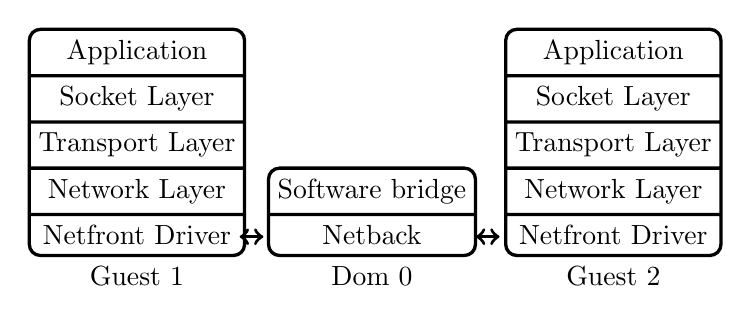
\begin{tikzpicture}
      [domU/.style={
           rectangle split,
           rectangle split parts=5,
           rounded corners,
           draw=black, very thick,
           text centered,
           anchor=five
         },
       dom0/.style={
           rectangle split,
           rectangle split parts=2,
           rounded corners,
           draw=black, very thick,
           text centered,
           anchor=two
         },
       ]
    \node [domU, label=below:Guest 1] (dom1) at (-3,0) {
      Application
      \nodepart{two}
      Socket Layer
      \nodepart{three}
      Transport Layer
      \nodepart{four}
      Network Layer
      \nodepart{five}
      Netfront Driver
    };
    
    \node [domU, label=below:Guest 2] (dom2) at (3.05,0) {
      Application
      \nodepart{two}
      Socket Layer
      \nodepart{three}
      Transport Layer
      \nodepart{four}
      Network Layer
      \nodepart{five}
      Netfront Driver
    };

    \node [dom0, label=below:Dom 0] (dom0) at (0.55,0) {
      Software bridge
      \nodepart{two}
      Netback
    };

    \path (-0.5,0.1) edge [draw=black, very thick, <->] (-0.2,0.1);
    \path (2.5,0.1) edge [draw=black, very thick, <->] (2.8,0.1);
    
  \end{tikzpicture}
  \caption{Normal IP architecture of Xen domUs}
  \label{xen_normal_architecture}
\end{figure}


Xen offers an way to directly share memory between hosts.
Using such dedicated memory should allow to create channels between virtual hosts with only a few data copies and little to no kernel involvement.

\subsection{Related work}




\subsection{Our work}

This projects tries tobuild a channel between two virtual hosts better than the existing solutions. For that purpose, the channel directly puts the shared memory into the userspace, reducing to the minimum the number of system calls (and thus context switching) and also transferring the data with only to successive copies. Our implementation is divided into two parts:

\begin{figure}[h]
  \centering
  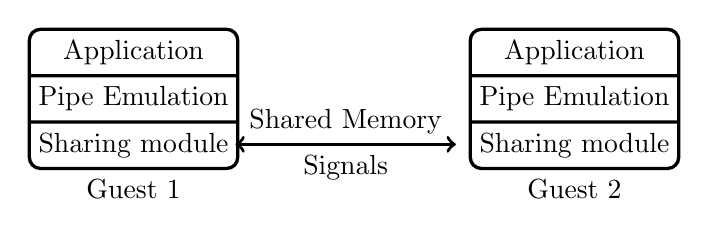
\begin{tikzpicture}
      [domU/.style={
           rectangle split,
           rectangle split parts=3,
           rounded corners,
           draw=black, very thick,
           text centered,
           anchor=three
         },
       ]
    \node [domU, label=below:Guest 1] (dom1) at (-2.8,0) {
      Application
      \nodepart{two}
      Pipe Emulation
      \nodepart{three}
      Sharing module
    };
    
    \node [domU, label=below:Guest 2] (dom2) at (2.8,0) {
      Application
      \nodepart{two}
      Pipe Emulation
      \nodepart{three}
      Sharing module
    };

    \path (-0.3,0.1) edge [draw=black, very thick, <->] node [above] {Shared Memory} node [below] {Signals} (2.5,0.1);
    
  \end{tikzpicture}
  \caption{Optimised channel using shared memory and signals}
  \label{xen_shm}
\end{figure}


The Xen shared memory tool, a kernel module, provides a way of sharing memory between two user-spaces of possibly different virtual machines on the same Xen hypervisor.
For performance purposes and because of possible dead-locks, this module also contains a set of particular operations that needs kernel context switching but that provide signals between
the two clients.

The second part, a user space library on top of the kernel module interface, provides read and write operations like any unidirectional channel abstraction. It abstracts the inner work that transform memory into a unidirectional channel, using as few system calls as possible.

The next parts of this report are dedicated to the explanation, in more details, of those two different parts.

\section{Shared memory device}

\subsection{Xen shared memory}



\subsection{Create shared memory}



\subsection{Map memory into user-space}



\subsection{Event channel}



\subsection{Closure}









\section{Shared memory based circular buffer}

\subsection{Principles}



\subsection{Optimizations}



\subsection{Closure and dead-lock avoidance}






\section{Evaluation}


\subsection{Configuration}

\subsection{Throughput}

\begin{figure}[h]
\centering
\begin{tikzpicture}
    \begin{semilogxaxis}[
        xlabel=Buffer size (KiB),
        ylabel=Throughput (Gbps),
        legend style={nodes=right},
        legend pos= north west,
        scaled ticks=false, 
        compat=1.3
        ]
        
    \addplot table [ x index=0,y index=1] {plots/bandwidth.txt};
    \addlegendentry{Xen pipe}
    
    \addplot table[ x index=0,y index=3] {plots/bandwidth.txt};
    \addlegendentry{Stressed Xen pipe}
    
    \addplot table[ x index=0,y index=2] {plots/bandwidth.txt};
    \addlegendentry{TCP}
    
    
    \end{semilogxaxis}
\end{tikzpicture}
\caption{Comparison between Xen pipe and TCP throughputs for different buffer sizes}
\label{shm_size}
\end{figure}


\begin{figure}[h]
\centering
\begin{tikzpicture}
    \begin{semilogxaxis}[
        xlabel=Message size (Bytes),
        ylabel=Throughput (Gbps),
        legend style={nodes=right},
        legend pos= north west,
        scaled ticks=false, 
        compat=1.3
        ]
        
        
        \addplot table[x index=0,y index=4] {plots/messageSize.txt};
    \addlegendentry{XenPipe: 60}
        
      \addplot table[ x index=0,y index=3] {plots/messageSize.txt};
    \addlegendentry{XenPipe: 20}  
        
        
     \addplot table[  x index=0,y index=2] {plots/messageSize.txt};
    \addlegendentry{XenPipe: 5}   
        
    \addplot table[  x index=0,y index=1] {plots/messageSize.txt};
    \addlegendentry{XenPipe: 1}
    
    
    \addplot [smooth,dashed,mark=*,orange] table[  x index=0,y index=5] {plots/messageSize.txt};
    \addlegendentry{XWay}
    
    \addplot [smooth,dashed,mark=square*, violet]  table[  x index=0,y index=7,orange] {plots/messageSize.txt};
    \addlegendentry{XenSocket}

    \addplot [smooth,dashed,mark=x, magenta] table[  x index=0,y index=6] {plots/messageSize.txt};
    \addlegendentry{XenLoop}
   
    \end{semilogxaxis}
\end{tikzpicture}
\caption{Throughput of Xen Pipe with different shared memory sizes (indicated in pages) and other state-of-the-art solutions with respect to the message size}
\label{msg_size}
\end{figure}


\subsection{Delays}

\subsection{Simultaneous transfers}



\begin{figure}[h]
\centering
\begin{tikzpicture}
    \begin{semilogyaxis}[
        xlabel=Number of parallel flows,
        ylabel=Throughput (Mbps),
        legend style={nodes=right},
        legend pos= south west,
        scaled ticks=false, 
        y tick label style={/pgf/number format/.cd,sci,precision=5},
        compat=1.3,
        ]
        
        
        \addplot [blue,mark=x] table[x index=0,y index=1] {plots/multi.txt};
    \addlegendentry{Total throughput}
        
     
    
    \addplot [smooth, red] table[x index=0,y index=8] {plots/multi.txt};
    \addlegendentry{Optimal sharing}
    
     %\addplot [smooth, black] table[x index=0,y index=5] {multi.txt};
    %\addlegendentry{Median value}
    
    %\addplot [smooth, gray] table[x index=0,y index=6] {multi.txt};
    
    %\addplot [smooth, gray] table[x index=0,y index=7] {multi.txt};
       
    %\addplot [smooth, lightgray] table[x index=0,y index=3] {multi.txt};
    
    %\addplot [smooth, lightgray] table[x index=0,y index=4] {multi.txt};
    
    \addplot [box plot median] table {plots/boxes.txt};
    \addplot [box plot box] table {plots/boxes.txt};
    \addplot [box plot top whisker] table {plots/boxes.txt};
    \addplot [box plot bottom whisker] table {plots/boxes.txt};
    \addlegendentry{Values distribution}

    
    \end{semilogyaxis}
\end{tikzpicture}
\caption{Throughputs of multiple parallel flows (60 shared pages per transfert - messages of 32KiB - average value over more than 20 seconds). The dark line corresponds to the median value. 
Gray lines correspond to first and last decile. Light gray lines correspond to the maximum and minimum values}
\label{simult_flows}
\end{figure}





\section{Conclusion}

\subsection{Contributions}


\subsection{Possible improvements}







 
% if have a single appendix:
%\appendix[Proof of the Zonklar Equations]
% or
%\appendix  % for no appendix heading
% do not use \section anymore after \appendix, only \section*
% is possibly needed

% use appendices with more than one appendix
% then use \section to start each appendix
% you must declare a \section before using any
% \subsection or using \label (\appendices by itself
% starts a section numbered zero.)
%


%\appendices
%\section{Figures}
%Appendix one text goes here.




% you can choose not to have a title for an appendix
% if you want by leaving the argument blank

%Appendix two text goes here.


% use section* for acknowledgement
%\section*{Acknowledgment}
%
%
%The authors would like to thank...



% Can use something like this to put references on a page
% by themselves when using endfloat and the captionsoff option.
\ifCLASSOPTIONcaptionsoff
  \newpage
\fi



\begin{thebibliography}{1}

\bibitem{IEEEhowto:kopka}
Xiaolan Zhang et al., \emph{XenSocket: A High-Throughput Interdomain Transport for Virtual Machines}, Middleware '07.

\bibitem{IEEEhowto:kopka}
Kangho Kim et al., \emph{Inter-domain Socket Communications Supporting High Performance and Full Binary Compatibility on Xen}, VEE '08.

\bibitem{IEEEhowto:kopka}
Jian Wang et al., \emph{XenLoop : A Transparent High Performance Inter-VM Network Loopback}, HPDC '08.

\end{thebibliography}





% that's all folks
\end{document}


